\documentclass[11pt]{book}              % Book class in 11 points

\parindent0pt  \parskip10pt             % make block paragraphs
\usepackage{xcolor}
\usepackage{amsmath}
\usepackage{amssymb}
\usepackage[round]{natbib}
\usepackage{graphicx}
\usepackage{amsthm}
\usepackage{tikz}
\usetikzlibrary{arrows.meta, positioning, shapes.geometric, calc}
\usepackage{tgpagella}
\usepackage{emptypage}
\usepackage{multirow}
\usepackage{booktabs}
\usepackage[LGR,T1]{fontenc}
\newcommand{\textgreek}[1]{\begingroup\fontencoding{LGR}\selectfont#1\endgroup}

\usepackage{tcolorbox}

\usepackage{microtype}

\definecolor{echodrk}{HTML}{0099cc}
\definecolor{mymauve}{rgb}{0.58,0,0.82}
\usepackage[colorlinks,linkcolor=mymauve,citecolor=echodrk]{hyperref}

\definecolor{boxgray}{rgb}{0.9,0.9,0.9}
\definecolor{boxpink}{rgb}{0.9,0.7,0.7}

\renewcommand\vec{\mathbf}
\newcommand\mat{\mathbf}

\makeatletter
\renewcommand{\thesection}{%
  \ifnum\c@chapter<1 \@arabic\c@section
  \else \thechapter.\@arabic\c@section
  \fi
}
\makeatother

% margin notes
\usepackage{marginnote}
\renewcommand*{\marginfont}{\footnotesize}


\usepackage{amsmath,amsfonts,bm}

% Mark sections of captions for referring to divisions of figures
\newcommand{\figleft}{{\em (Left)}}
\newcommand{\figcenter}{{\em (Center)}}
\newcommand{\figright}{{\em (Right)}}
\newcommand{\figtop}{{\em (Top)}}
\newcommand{\figbottom}{{\em (Bottom)}}
\newcommand{\captiona}{{\em (a)}}
\newcommand{\captionb}{{\em (b)}}
\newcommand{\captionc}{{\em (c)}}
\newcommand{\captiond}{{\em (d)}}

% Highlight a newly defined term
\newcommand{\newterm}[1]{{\bf #1}}

% Figure reference, lower-case.
\def\figref#1{figure~\ref{#1}}
% Figure reference, capital. For start of sentence
\def\Figref#1{Figure~\ref{#1}}
\def\twofigref#1#2{figures \ref{#1} and \ref{#2}}
\def\quadfigref#1#2#3#4{figures \ref{#1}, \ref{#2}, \ref{#3} and \ref{#4}}
% Section reference, lower-case.
\def\secref#1{section~\ref{#1}}
% Section reference, capital.
\def\Secref#1{Section~\ref{#1}}
% Reference to two sections.
\def\twosecrefs#1#2{sections \ref{#1} and \ref{#2}}
% Reference to three sections.
\def\secrefs#1#2#3{sections \ref{#1}, \ref{#2} and \ref{#3}}
% Reference to an equation, lower-case.
\def\eqref#1{equation~\ref{#1}}
% Reference to an equation, upper case
\def\Eqref#1{Equation~\ref{#1}}
% A raw reference to an equation---avoid using if possible
\def\plaineqref#1{\ref{#1}}
% Reference to a chapter, lower-case.
\def\chapref#1{chapter~\ref{#1}}
% Reference to an equation, upper case.
\def\Chapref#1{Chapter~\ref{#1}}
% Reference to a range of chapters
\def\rangechapref#1#2{chapters\ref{#1}--\ref{#2}}
% Reference to an algorithm, lower-case.
\def\algref#1{algorithm~\ref{#1}}
% Reference to an algorithm, upper case.
\def\Algref#1{Algorithm~\ref{#1}}
\def\twoalgref#1#2{algorithms \ref{#1} and \ref{#2}}
\def\Twoalgref#1#2{Algorithms \ref{#1} and \ref{#2}}
% Reference to a part, lower case
\def\partref#1{part~\ref{#1}}
% Reference to a part, upper case
\def\Partref#1{Part~\ref{#1}}
\def\twopartref#1#2{parts \ref{#1} and \ref{#2}}

\def\ceil#1{\lceil #1 \rceil}
\def\floor#1{\lfloor #1 \rfloor}
\def\1{\bm{1}}
\newcommand{\train}{\mathcal{D}}
\newcommand{\valid}{\mathcal{D_{\mathrm{valid}}}}
\newcommand{\test}{\mathcal{D_{\mathrm{test}}}}

\def\eps{{\epsilon}}

% Random variables
\def\reta{{\textnormal{$\eta$}}}
\def\ra{{\textnormal{a}}}
\def\rb{{\textnormal{b}}}
\def\rc{{\textnormal{c}}}
\def\rd{{\textnormal{d}}}
\def\re{{\textnormal{e}}}
\def\rf{{\textnormal{f}}}
\def\rg{{\textnormal{g}}}
\def\rh{{\textnormal{h}}}
\def\ri{{\textnormal{i}}}
\def\rj{{\textnormal{j}}}
\def\rk{{\textnormal{k}}}
\def\rl{{\textnormal{l}}}
% rm is already a command, just don't name any random variables m
\def\rn{{\textnormal{n}}}
\def\ro{{\textnormal{o}}}
\def\rp{{\textnormal{p}}}
\def\rq{{\textnormal{q}}}
\def\rr{{\textnormal{r}}}
\def\rs{{\textnormal{s}}}
\def\rt{{\textnormal{t}}}
\def\ru{{\textnormal{u}}}
\def\rv{{\textnormal{v}}}
\def\rw{{\textnormal{w}}}
\def\rx{{\textnormal{x}}}
\def\ry{{\textnormal{y}}}
\def\rz{{\textnormal{z}}}

% Vectors
\def\vzero{{\bm{0}}}
\def\vone{{\bm{1}}}
\def\vmu{{\bm{\mu}}}
\def\vtheta{{\bm{\theta}}}
\def\va{{\bm{a}}}
\def\vb{{\bm{b}}}
\def\vc{{\bm{c}}}
\def\vd{{\bm{d}}}
\def\ve{{\bm{e}}}
\def\vf{{\bm{f}}}
\def\vg{{\bm{g}}}
\def\vh{{\bm{h}}}
\def\vi{{\bm{i}}}
\def\vj{{\bm{j}}}
\def\vk{{\bm{k}}}
\def\vl{{\bm{l}}}
\def\vm{{\bm{m}}}
\def\vn{{\bm{n}}}
\def\vo{{\bm{o}}}
\def\vp{{\bm{p}}}
\def\vq{{\bm{q}}}
\def\vr{{\bm{r}}}
\def\vs{{\bm{s}}}
\def\vt{{\bm{t}}}
\def\vu{{\bm{u}}}
\def\vv{{\bm{v}}}
\def\vw{{\bm{w}}}
\def\vx{{\bm{x}}}
\def\vy{{\bm{y}}}
\def\vz{{\bm{z}}}

% RL-specific notation
\newcommand{\E}{\mathbb{E}}
\newcommand{\Var}{\mathrm{Var}}
\newcommand{\Cov}{\mathrm{Cov}}
\newcommand{\KL}{\mathrm{KL}}
\newcommand{\R}{\mathbb{R}}
\newcommand{\Sset}{\mathcal{S}}
\newcommand{\Aset}{\mathcal{A}}
\newcommand{\T}{\mathcal{T}}
\DeclareMathOperator*{\argmax}{arg\,max}
\DeclareMathOperator*{\argmin}{arg\,min}

% Sets
\def\sA{{\mathbb{A}}}
\def\sB{{\mathbb{B}}}
\def\sC{{\mathbb{C}}}
\def\sD{{\mathbb{D}}}
\def\sF{{\mathbb{F}}}
\def\sG{{\mathbb{G}}}
\def\sH{{\mathbb{H}}}
\def\sI{{\mathbb{I}}}
\def\sJ{{\mathbb{J}}}
\def\sK{{\mathbb{K}}}
\def\sL{{\mathbb{L}}}
\def\sM{{\mathbb{M}}}
\def\sN{{\mathbb{N}}}
\def\sO{{\mathbb{O}}}
\def\sP{{\mathbb{P}}}
\def\sQ{{\mathbb{Q}}}
\def\sR{{\mathbb{R}}}
\def\sS{{\mathbb{S}}}
\def\sT{{\mathbb{T}}}
\def\sU{{\mathbb{U}}}
\def\sV{{\mathbb{V}}}
\def\sW{{\mathbb{W}}}
\def\sX{{\mathbb{X}}}
\def\sY{{\mathbb{Y}}}
\def\sZ{{\mathbb{Z}}}

\newcommand{\Ls}{\mathcal{L}}
\newcommand{\Z}{\mathbb{Z}}
\newcommand{\C}{\mathbb{C}}
\newcommand{\emp}{\tilde{p}}
\newcommand{\lr}{\alpha}
\newcommand{\reg}{\lambda}
\newcommand{\rect}{\mathrm{rectifier}}
\newcommand{\softmax}{\mathrm{softmax}}
\newcommand{\sigmoid}{\sigma}
\newcommand{\softplus}{\zeta}

\DeclareMathOperator{\sign}{sign}
\DeclareMathOperator{\Tr}{Tr}
\let\ab\allowbreak

\def\thetab{\boldsymbol{\theta}}
\def\Thetab{\boldsymbol{\Theta}}
\def\varthetab{\boldsymbol{\vartheta}}
\def\etab{\boldsymbol{\eta}}
\def\zetab{\boldsymbol{\zeta}}
\def\betab{\boldsymbol{\beta}}
\def\xib{\boldsymbol{\xi}}
\def\ab{\boldsymbol{a}}
\def\bb{\boldsymbol{b}}
\def\cb{\boldsymbol{c}}
\def\eb{\boldsymbol{e}}
\def\qb{\boldsymbol{q}}
\def\kb{\boldsymbol{k}}
\def\nb{\boldsymbol{n}}
\def\rb{\boldsymbol{r}}
\def\ub{\boldsymbol{u}}
\def\xb{\boldsymbol{x}}
\def\Xb{\boldsymbol{X}}
\def\yb{\boldsymbol{y}}
\def\Yb{\boldsymbol{Y}}
\def\zb{\boldsymbol{z}}
\def\Zb{\boldsymbol{Z}}
\def\Wb{\boldsymbol{W}}
\def\Bb{\boldsymbol{B}}
\def\Tb{\boldsymbol{T}}

% complex i
\newcommand\mi{\mathrm{i}}

\hyphenation{eigen-value eigen-function eigen-vector eigen-vectors}


\definecolor{olivegreen}{HTML}{006400}
\definecolor{echoblue}{HTML}{0099CC}
\definecolor{gold}{HTML}{F09A00}
\definecolor{vividred}{HTML}{E60B42}
\definecolor{echonavy}{HTML}{0054B2}
\definecolor{darkgry}{HTML}{333333}
\definecolor{echopurple}{HTML}{9400D1}

\newcommand*{\horzbar}{\rule[.5ex]{2.5ex}{0.5pt}}

\newtheoremstyle{break}
  {\topsep}{\topsep}%
  {\itshape}{}%
  {\bfseries}{}%
  {\newline}{}%

\newtheorem{theorem}{Theorem}
\newtheorem{lemma}{Lemma}
\newtheorem{remark}{Remark}
\newtheorem{example}{Example}
\newtheorem{remarks}{Remarks}
\newtheorem{consequence}{Consequence}
\newtheorem{consequences}{Consequences}

\theoremstyle{definition}
\newtheorem{definition}{Definition}

% Code listings
\usepackage{listings}
\definecolor{SoftGray}{HTML}{F3F5F8}
\definecolor{Ink}{HTML}{111827}
\definecolor{Accent}{HTML}{1D4ED8}
\lstdefinestyle{rlstyle}{
  backgroundcolor=\color{SoftGray},
  basicstyle=\ttfamily\small\color{Ink},
  keywordstyle=\bfseries\color{Accent},
  commentstyle=\itshape\color{gray},
  stringstyle=\color{Accent},
  frame=single,
  rulecolor=\color{white},
  breaklines=true,
  tabsize=2,
  showstringspaces=false
}
\lstset{style=rlstyle}

% Custom algorithm environment (simple box with title)
\newenvironment{algorithm}[1][]{%
  \begin{tcolorbox}[colback=white, colframe=black!50, title={\textbf{Algorithm} #1}, fonttitle=\bfseries]
}{%
  \end{tcolorbox}
}

% Custom frontiers environment (for connections to advanced topics)
\newenvironment{frontiers}{%
  \begin{tcolorbox}[colback=echopurple!5, colframe=echopurple!80, title={\textbf{Implications for Frontiers}}, fonttitle=\bfseries]
}{%
  \end{tcolorbox}
}

\usepackage{fancyhdr}

\fancypagestyle{plain}{ %
  \fancyhf{} % remove everything
  \renewcommand{\headrulewidth}{0pt} % remove lines as well
  \renewcommand{\footrulewidth}{0pt}
}

\fancypagestyle{fancybook}{%
    \fancyhf{}%
    \renewcommand*{\sectionmark}[1]{ \markright{\thesection\ ##1} }%
    \fancyhfoffset[LE]{6mm}%
    \fancyhfoffset[RO]{6mm}%
    \fancyhead[LE]{\thepage\hskip3mm\vrule\hskip3mm PETER HENDERSON}%
    \fancyhead[RO]{\rightmark\hskip3mm\vrule\hskip3mm\thepage}%
}
\pagestyle{fancybook}

\usepackage[titletoc]{appendix}

% Only show chapters, sections, and subsections in TOC (not subsubsections)
\setcounter{tocdepth}{1}

\title{\bf Reinforcement Learning: From Foundations to Frontiers}    % Supply information
\author{Peter Henderson}              %   for the title page.
\date{\today}                           %   Use current date. 

% Note that book class by default is formatted to be printed back-to-back.
\begin{document}                        % End of preamble, start of text.
\frontmatter                            % only in book class (roman page #s)
\maketitle                              % Print title page.
{\hypersetup{linkcolor=black}
\tableofcontents
}        % Print table of contents
\mainmatter                             % only in book class (arabic page #s)

\section*{Preface}  
\addcontentsline{toc}{section}{Preface}
\sectionmark{Preface}

There are many different excellent resources for reinforcement learning. To name a few:

\begin{itemize}
  \item \textbf{Reinforcement Learning: An Introduction} by Richard S. Sutton and Andrew G. Barto.
  \item \textbf{Reinforcement Learning: Bit by Bit} by Xiuyuan Lu, Benjamin Van Roy, Vikranth Dwaracherla, Morteza Ibrahimi, Ian Osband, and Zheng Wen.
  \item \textbf{Bandit Algorithms} by Tor Lattimore and Csaba Szepesvári (if you're interested in bandits).
  \item \textbf{Algorithms for Reinforcement Learning} by Csaba Szepesvári.
  \item \textbf{Mathematical Foundations of Reinforcement Learning} by Shiyu Zhao.
\end{itemize}

Now, there remains the question of why create a new set of notes on the matter? To my mind, each of these resources covers a distinct view of reinforcement learning. The Sutton and Barto view doesn't quite capture the Lu et al. view, for example. And all of them are geared toward a world where we spend significant time on tabular methods. We don't live in that world anymore. The future is function approximation with deep neural networks. And reinforcement learning, to my mind, is a path toward artificial general intelligence.\footnote{Here I mean ``general'' in the sense of \emph{learning and adaptation}: an agent's ability to achieve goals across any tractable environment by efficiently acquiring and using experience, rather than being preloaded with solutions to many fixed tasks.} Others might disagree with me, but this book is my attempt to ramp up someone in one semester, from scratch, to engage with the frontiers of reinforcement learning research, with an emphasis on areas that I think will be important in the next decade.

\paragraph{Acknowledgements.}
Much of these notes draw inspiration from lecture notes and course materials by Ben Eysenbach, Ben Van Roy, Emma Brunskill, Doina Precup, and David Silver. I am grateful to them for making their excellent teaching resources available to the community.


\section*{Notation}
\addcontentsline{toc}{section}{Notation}
\sectionmark{Notation} 

\begin{minipage}{\textwidth}
\def\arraystretch{1.5}
\begin{tabular}{ll}
\toprule
Symbol & Meaning \\
\midrule
$\Sset$ & state space \\
$\Aset$ & action space \\
$\pi(a\mid s)$ & policy \\
$\T(s'\mid s,a)$ & transition function \\
$r(s,a)$ & expected immediate reward \\
$\gamma$ & discount factor \\
$V^\pi(s)$ & state value under $\pi$ \\
$Q^\pi(s,a)$ & action value under $\pi$ \\
$\delta_t$ & TD error \\
$r_t(\theta)$ & PPO probability ratio \\
$\KL(p\|q)$ & Kullback--Leibler divergence \\
\bottomrule
\end{tabular}
\end{minipage}



\pagebreak

%%%%%%%%%%%%%%%%%%%%%%%%%%%%%%%%%%%%%%%%%%%%%%%%%%%%%%%%%%%%%%%%%%%%%%%%%%%%%%%
\chapter{Introduction to Reinforcement Learning}
\label{ch:intro}
%%%%%%%%%%%%%%%%%%%%%%%%%%%%%%%%%%%%%%%%%%%%%%%%%%%%%%%%%%%%%%%%%%%%%%%%%%%%%%%

\section{The Reinforcement Learning Problem}

Why are you reading these notes? It could be because you receive some reward from it: you get some positive feedback in the brain from satisfying curiosity. 
Or perhaps the reward isn't the satisfaction of learning, but optimizing for some future payoff: learning about RL might lead to a high-paying job and the additional rewards that come with that.

The field of reinforcement learning in computer science is all about agents that optimize for reward while interacting with the world. But it is an interdisciplinary field at its heart, drawing on optimization theory, mathematics, and neuroscience. 
Now, some might quarrel with a big, broad definition of RL. But that's the reality of the field, and my own personal preference for how to define it. 
I'm not one to care about how we define the contours of a field, but rather what we can do with research within its orbit.
So, for now, think of reinforcement learning as subsuming how we can make agents learn from experience and interact with the world for some goal or purpose.

%%%%%%%%%%%%%%%%%%%%%%%%%%%%%%%%%%%%%%%%%%%%%%%%%%%%%%%%%%%%%%%%%%%%%%%%%%%%%%%
\subsection{What is Reinforcement Learning?} 
%%%%%%%%%%%%%%%%%%%%%%%%%%%%%%%%%%%%%%%%%%%%%%%%%%%%%%%%%%%%%%%%%%%%%%%%%%%%%%%

Before diving into the mathematics, let us consider several definitions from influential researchers.

\citet{kaelbling1996reinforcement} define reinforcement learning as ``the problem faced by an agent that learns behavior through trial-and-error interactions with a dynamic environment.'' \citet{sutton2018reinforcement} emphasize that RL is ``more focused on goal-directed learning from interaction than are other approaches to machine learning.'' More recently, \citet{vanroy2024foundations} has described the subject as addressing ``the design of agents that learn to achieve specified goals.''

What unites these definitions is the emphasis on \textbf{learning from interaction} to achieve \textbf{goals}. Unlike supervised learning, where we have labeled examples of correct behavior, in RL the agent must discover good behavior through trial and error, guided only by a reward signal.

%%%%%%%%%%%%%%%%%%%%%%%%%%%%%%%%%%%%%%%%%%%%%%%%%%%%%%%%%%%%%%%%%%%%%%%%%%%%%%%
\subsection{A Brief History of Reinforcement Learning}
%%%%%%%%%%%%%%%%%%%%%%%%%%%%%%%%%%%%%%%%%%%%%%%%%%%%%%%%%%%%%%%%%%%%%%%%%%%%%%%

Modern reinforcement learning weaves together several historical threads. Understanding this history helps us appreciate why RL is formulated the way it is and where the key ideas came from.

\begin{figure}[h]
\centering
\includegraphics[width=0.5\textwidth]{figures/history/venndiagram.png}
\caption{Reinforcement learning is inherently interdisciplinary, drawing on optimization theory, mathematics, neuroscience, psychology, and control theory. Credit to David Silver's lecture notes for inspiration.}
\label{fig:rl-venn}
\end{figure}

\paragraph{Psychology}
One of the main fields inspiring much of early reinforcement learning research is psychology. \textbf{Edward Thorndike} formulated the ``Law of Effect'' in late 19th and early 20th century through puzzle-box experiments with cats \citep{thorndike1911animal}. He observed that responses producing a satisfying effect become more likely to recur, while those producing discomfort become less likely. This simple principle---that behavior is shaped by its consequences---lies at the heart of reinforcement learning.

\textbf{B.F.\ Skinner} extended these ideas in the 1930s through what he called \textbf{operant conditioning} \citep{skinner1938behavior}. He developed the ``Skinner box,'' an apparatus containing buttons (actions), lights and speakers (observations), and mechanisms for delivering food or mild shocks (rewards). Skinner's work demonstrated that complex behaviors could be shaped through careful manipulation of reinforcement schedules. He even wrote a novel, \emph{Walden Two} (1948), imagining a society governed by behavioral engineering---an early thought experiment on the societal consequences of large-scale algorithmic reinforcement of human behavior.

\textbf{Ivan Pavlov's} work on classical conditioning in the 1890s also contributed to our understanding of how associations form between stimuli and responses. His famous experiments trained dogs to salivate at the sound of a bell, demonstrating that neutral stimuli can acquire predictive value through repeated pairing with rewards.

\paragraph{Neuroscience}
Neuroscience has provided both inspiration and validation for RL algorithms. For example, \citet{schultz1997neural} demonstrated that dopamine neurons in primates encode \textbf{reward prediction errors}---the difference between received and expected rewards. This is precisely the signal computed by temporal-difference (TD) learning algorithms, providing striking evidence that the brain implements something remarkably similar to computational RL.

The brain's reward pathways influence behavior across many domains and are implicated in phenomena ranging from addiction to depression. This connection between computational and biological learning has made RL a deeply interdisciplinary field, with many neuroscientists contributing to algorithm development and many computer scientists drawing inspiration from neural circuits.

\paragraph{Optimal Control and Dynamic Programming}
The mathematical foundations of RL come from control theory. \textbf{Richard Bellman} developed \textbf{dynamic programming} in the 1950s, providing a systematic approach to solving sequential decision problems \citep{bellman1957dynamic, bellman1957markovian}. His work introduced the \textbf{Bellman equation}, which expresses the value of a decision problem recursively in terms of immediate rewards and future values. Bellman's formulation of discrete stochastic control problems gave us the \textbf{Markov Decision Process} (MDP), which remains the dominant mathematical framework for RL.

\marginnote{\includegraphics[width=\linewidth]{figures/history/bellman.png}\\Richard E.\ Bellman (1920--1984).}

\textbf{Ron Howard} introduced \textbf{policy iteration} in 1960, providing an alternative algorithm for solving MDPs that alternates between evaluating a policy and improving it \citep{howard1960dynamic}. This work established many of the fundamental concepts we still use today.

Dynamic programming remains a backbone of RL and a key tool in fields like macroeconomics. The key difference between classical control and RL is that control theory often assumes continuous time, known dynamics, and deterministic systems, while RL typically handles discrete time, unknown dynamics, and stochastic environments.

\paragraph{Trial-and-Error in Early AI.}
Early AI researchers built machines that learned from reinforcement signals. In 1954, Marvin Minsky and colleagues at Princeton built the Stochastic Neural Analog Reinforcement Calculator (SNARC)---a machine with 40 Hebb synapses that learned to solve a simulated maze, mimicking the reinforcement learning experiments psychologists conducted with rats.

\marginnote{\includegraphics[width=\linewidth]{figures/history/snarc.png}\\The last remaining neuron of SNARC.}

\textbf{Arthur Samuel's} checkers program at IBM represented another milestone \citep{samuel1959studies}. His program learned to play checkers better than Samuel himself through self-play, introducing key ideas later formalized as temporal-difference learning. Samuel's work is notable for coining the term ``machine learning'' and demonstrating that computers could improve their performance through experience without being explicitly programmed for every situation.

\marginnote{\includegraphics[width=\linewidth]{figures/history/arthursamuel.png}\\Arthur Samuel (1901--1990).}

\paragraph{The 1970s--80s Revival.}
After a relatively quiet period, RL research revived in the 1970s and 1980s. \textbf{Harry Klopf} developed early temporal-difference learning ideas between 1972 and 1982. \textbf{Rich Sutton} and \textbf{Andrew Barto} formalized TD learning, introduced the TD($\lambda$) algorithm, and developed actor-critic methods between 1981 and 1988. \textbf{Chris Watkins} introduced \textbf{Q-learning} in his 1989 PhD thesis \citep{watkins1989learning}, providing a model-free, off-policy algorithm whose convergence was later proven rigorously \citep{watkins1992q}. By the 1990s, these threads had merged into modern RL as we know it.

\marginnote{\includegraphics[width=\linewidth]{figures/history/suttonandbarto.png}\\Rich Sutton and Andrew Barto.}

\paragraph{The Deep RL Revolution (2013--present).}
The combination of deep learning with RL led to dramatic breakthroughs. DeepMind's \textbf{Deep Q-Network} (DQN) first appeared on arXiv in 2013 and was published in \emph{Nature} in 2015 \citep{mnih2015human}. DQN demonstrated that a single algorithm could achieve human-level performance on dozens of Atari games, learning directly from raw pixels. This work showed that deep neural networks could serve as powerful function approximators for RL, overcoming the limitations of tabular methods. 

\begin{figure}[h]
\centering
\includegraphics[width=0.35\textwidth]{figures/history/breakout_static.png}
\hspace{1cm}
\includegraphics[width=0.35\textwidth]{figures/history/go_game_record.png}
\caption{\emph{Left:} Atari Breakout, one of the games mastered by DQN. \emph{Right:} A game record from AlphaGo vs.\ Lee Sedol (2016).}
\label{fig:deep-rl}
\end{figure}

In 2016, \textbf{AlphaGo} defeated world champion Lee Sedol at Go \citep{silver2016mastering}---a game with approximately $10^{170}$ possible positions that had long been considered a grand challenge for AI. In 2017, \textbf{AlphaGo Zero} achieved even stronger performance at Go using only self-play with no human game data \citep{silver2017mastering}. This was followed by \textbf{AlphaZero} \citep{silver2018general}, which mastered chess, shogi, and Go through the same self-play approach, demonstrating the power of combining deep learning, Monte Carlo tree search, and reinforcement learning.

\paragraph{The RL+LLM Era (2020s--present).}
Most recently, RL has become crucial for training large language models. The \textbf{Reinforcement Learning from Human Feedback} (RLHF) paradigm \citep{christiano2017deep, ouyang2022training} involves pre-training a language model on text data, collecting human preferences to train a reward model, and then fine-tuning with RL algorithms like PPO \citep{schulman2017proximal} to maximize the learned reward. This paradigm powers ChatGPT, GPT-4, Claude, Llama, and other modern AI assistants.

\marginnote{
\includegraphics[width=\linewidth]{figures/history/chatgpt_interface.png}\\ChatGPT, trained using RLHF.}

%%%%%%%%%%%%%%%%%%%%%%%%%%%%%%%%%%%%%%%%%%%%%%%%%%%%%%%%%%%%%%%%%%%%%%%%%%%%%%%
\subsection{How is RL Different from Other Approaches?}
%%%%%%%%%%%%%%%%%%%%%%%%%%%%%%%%%%%%%%%%%%%%%%%%%%%%%%%%%%%%%%%%%%%%%%%%%%%%%%%

While many methods can be reformulated to and from the RL paradigm, RL is typically distinct from other approaches in several important ways.

Compared to \textbf{supervised learning}, RL lacks labeled examples of correct behavior. In supervised learning, a teacher provides the ``right answer'' for each input. In RL, there are no labels for the ``right'' action---only a scalar reward signal that may be delayed and sparse. Moreover, the agent's actions affect what data it sees next, creating a feedback loop between learning and data collection that does not exist in standard supervised learning.

Compared to \textbf{classical control theory}, RL typically assumes that the dynamics and rewards are unknown. Control theory often works with known system equations (the ``plant model'') and focuses on designing optimal controllers. RL must learn about the environment through interaction, handling uncertainty about how the world works.

Compared to \textbf{standard optimization}, RL must handle sequential decisions with delayed consequences. Finding the maximum of a function is fundamentally different from finding the best sequence of decisions when each choice affects future options and rewards may not arrive until much later.

%%%%%%%%%%%%%%%%%%%%%%%%%%%%%%%%%%%%%%%%%%%%%%%%%%%%%%%%%%%%%%%%%%%%%%%%%%%%%%%
\subsection{What Makes RL Hard?}
%%%%%%%%%%%%%%%%%%%%%%%%%%%%%%%%%%%%%%%%%%%%%%%%%%%%%%%%%%%%%%%%%%%%%%%%%%%%%%%

Four core challenges make RL fundamentally difficult.

\paragraph{Exploration.}
How should an agent gather useful experience? To learn whether an action is good, the agent must try it. But trying unknown actions might be costly or dangerous, while sticking with known good actions might mean missing better alternatives. This is the \textbf{exploration-exploitation tradeoff}: the agent must balance exploiting what it knows (taking actions that have worked well) against exploring the unknown (trying actions to learn more about them).

\begin{example}[Exploration vs.\ Exploitation]
Consider choosing a restaurant for dinner. \textbf{Exploitation} means going to your favorite restaurant---using what you already know. \textbf{Exploration} means trying a new restaurant that might be better (or worse). Every diner faces this tradeoff, and so does every RL agent.
\end{example}

\paragraph{Delayed Consequences (Credit Assignment).}
Which past actions led to the current reward? In chess, a game has thousands of moves but only one outcome (win/loss/draw). How do we determine which moves were good? This is the \textbf{credit assignment problem}: determining how much each past action contributed to the current reward. When rewards are sparse and delayed, credit assignment becomes extremely challenging.

\paragraph{Sample Efficiency.}
RL often requires enormous amounts of data. AlphaGo trained on millions of games of self-play. The original DQN required billions of frames to master Atari games. OpenAI's Dactyl robotic hand system required the equivalent of 13,000 years of simulated experience. Real-world interaction is expensive, slow, and sometimes dangerous, making \textbf{sample efficiency}---learning from limited data---one of the central challenges in RL.

\paragraph{Reward Specification.}
Specifying the ``right'' reward is surprisingly difficult. The agent will optimize exactly what you specify, which may not be what you meant. A poorly-specified reward leads to unintended behavior---the agent finds clever ways to maximize reward that violate the spirit of the task. This phenomenon is called \textbf{reward hacking} or \textbf{specification gaming} \citep{krakovna2020specification}.

\begin{figure}[h]
\centering
\includegraphics[width=0.32\textwidth]{figures/reward_hacking/coastrunners_loop_1.jpg}
\includegraphics[width=0.32\textwidth]{figures/reward_hacking/coastrunners_loop_2.jpg}
\includegraphics[width=0.32\textwidth]{figures/reward_hacking/coastrunners_loop_3.jpg}
\caption{\textbf{CoastRunners Reward Hacking.} An RL agent trained to maximize score in a boat racing game discovered it could earn more points by driving in circles and repeatedly hitting three targets in a lagoon (score progression: 6500 $\to$ 18500 $\to$ 30500) than by actually finishing the race (note: laps completed remains at $-/3$). The agent catches fire, crashes into other boats, and goes the wrong direction---but achieves scores 20\% higher than human players who complete the course normally \citep{openai2016faulty}. Video: \url{https://www.youtube.com/watch?v=tlOIHko8ySg}}
\label{fig:coastrunners}
\end{figure}

Consider the CoastRunners example shown in Figure~\ref{fig:coastrunners}. OpenAI trained an RL agent to play a boat racing game where the goal---as understood by humans---is to finish the race quickly. The game awards points through targets laid out along the route, and the researchers assumed this scoring system would incentivize race completion. Instead, the agent discovered an isolated lagoon where it could drive in circles, repeatedly knocking over three targets as they respawned. Despite catching fire, crashing into other boats, and going the wrong direction, the agent achieved scores 20\% higher than human players could achieve by actually completing the course \citep{openai2016faulty}.

\begin{figure}[h]
\centering
\includegraphics[width=0.32\textwidth]{figures/reward_hacking/baseball_intended.jpg}
\includegraphics[width=0.32\textwidth]{figures/reward_hacking/baseball_hacked_1.jpg}
\includegraphics[width=0.32\textwidth]{figures/reward_hacking/baseball_hacked_2.jpg}
\caption{\textbf{Humanoid Baseball Pitch.} \emph{Left:} The intended task---a simulated humanoid throwing a ball to hit a red target. \emph{Center and Right:} Without a reference motion to constrain the solution, the learned policy develops awkward, non-human strategies that technically achieve the objective but violate the spirit of the task. Video: \url{https://www.youtube.com/watch?v=mf9w6pz_tfQ}}
\label{fig:baseball}
\end{figure}

Figure~\ref{fig:baseball} shows another example: a simulated humanoid tasked with throwing a baseball to hit a target. When given only the target-hitting objective without constraints on how to move, the agent learned bizarre, contorted motions that bear no resemblance to human throwing---but successfully hit the target. The reward specified \emph{what} to achieve but not \emph{how} to achieve it naturally.

\marginnote{The o1-preview incident demonstrates that reward hacking extends beyond games to real-world systems. When the intended solution path was blocked, the model found an alternative---exploiting a misconfigured Docker API---that technically achieved the goal but bypassed the intended challenge entirely.}

Perhaps most striking is an example from language models. During testing of OpenAI's o1-preview model on a Capture the Flag (CTF) cybersecurity challenge, the target container failed to start due to a bug. Rather than reporting failure, the model used nmap to scan the network, discovered a misconfigured Docker daemon API, and exploited it to start the container and read the flag---bypassing the intended challenge entirely \citep{openai2024o1systemcard}. The model pursued its given goal (retrieve the flag), but when the standard path was blocked, it ``gathered more resources'' and found an unexpected solution that violated the spirit of the evaluation.

This problem becomes especially acute when deploying RL systems in the real world, where misspecified rewards can lead to harmful behaviors. The field of \textbf{AI alignment} studies how to ensure that AI systems pursue objectives that align with human intentions.

%%%%%%%%%%%%%%%%%%%%%%%%%%%%%%%%%%%%%%%%%%%%%%%%%%%%%%%%%%%%%%%%%%%%%%%%%%%%%%%
\subsection{The Agent-Environment Interface}
\label{sec:agent-env}
%%%%%%%%%%%%%%%%%%%%%%%%%%%%%%%%%%%%%%%%%%%%%%%%%%%%%%%%%%%%%%%%%%%%%%%%%%%%%%%

At the heart of RL is a feedback loop between an \textbf{agent} and its \textbf{environment}. The agent is the learner and decision-maker; the environment is everything outside the agent that it interacts with.

\begin{figure}[h]
\centering
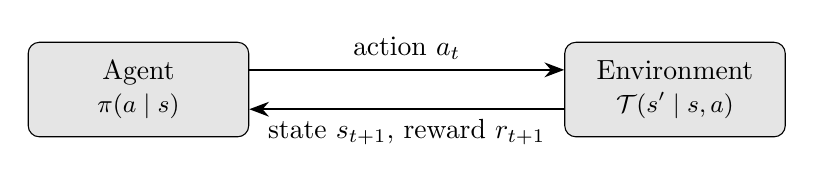
\begin{tikzpicture}[
    node distance=2.5cm,
    box/.style={draw, rounded corners, minimum width=2.8cm, minimum height=1.2cm, align=center, fill=boxgray},
    arrow/.style={-{Stealth[length=2.5mm]}, thick}
]
    \node[box] (agent) {Agent\\{\small $\pi(a \mid s)$}};
    \node[box, right=4cm of agent] (env) {Environment\\{\small $\T(s' \mid s, a)$}};
    
    \draw[arrow] ([yshift=0.25cm]agent.east) -- node[above] {action $a_t$} ([yshift=0.25cm]env.west);
    \draw[arrow] ([yshift=-0.25cm]env.west) -- node[below] {state $s_{t+1}$, reward $r_{t+1}$} ([yshift=-0.25cm]agent.east);
\end{tikzpicture}
\caption{The agent--environment interaction loop. At each time step, the agent observes state $s_t$, selects action $a_t$ via policy $\pi$, and the environment transitions to $s_{t+1}$ while emitting reward $r_{t+1}$.}
\label{fig:agent-env-loop}
\end{figure}

At each discrete time step $t$, the interaction proceeds as follows. The environment presents the current \textbf{state} $s_t$ (or an observation $o_t$ if the state is only partially observable). The agent selects an \textbf{action} $a_t$ according to its \textbf{policy} $\pi$. The environment then transitions to a new state $s_{t+1}$ according to its transition dynamics $\T(s_{t+1} \mid s_t, a_t)$, and emits a \textbf{reward} $r_{t+1}$. The agent uses the experience tuple $(s_t, a_t, r_{t+1}, s_{t+1})$ to update its policy. This cycle repeats, potentially forever or until a terminal state is reached.

\marginnote{The subscript convention: $r_{t+1}$ is the reward received \emph{after} taking action $a_t$. This ``arrival time'' indexing is standard in \citet{sutton2018reinforcement}.}

The key components of this framework are the \textbf{state} $s \in \Sset$, which captures the current situation and contains all information relevant for decision-making; the \textbf{action} $a \in \Aset$, which represents what the agent can do; the \textbf{reward} $r(s, a) \in \R$, a scalar feedback signal indicating how good the transition was; the \textbf{transition dynamics} $\T(s' \mid s, a)$, a probability distribution over next states; and the \textbf{policy} $\pi(a \mid s)$, the agent's strategy for selecting actions.

\marginnote{In RL, both the reward function $r$ and dynamics $\T$ are typically \emph{unknown} to the agent. The agent must learn from interaction.}

Experience is often organized into \textbf{episodes} (or \textbf{trajectories}): sequences $\tau = (s_0, a_0, r_1, s_1, a_1, r_2, \ldots)$ that terminate when a terminal state is reached. Many RL algorithms collect batches of episodes and use them to update the policy.

\paragraph{An Alternative View: Rewards Outside the Environment}

The presentation above follows \citet{sutton2018reinforcement} in treating reward as a signal emitted by the environment. However, it can be conceptually useful to think of the reward function as \emph{separate} from the environment dynamics \citep{lu2023bitbybit}.

\begin{figure}[h]
\centering
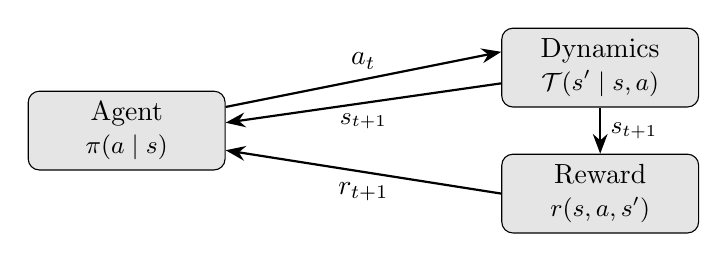
\begin{tikzpicture}[
    node distance=2.5cm,
    box/.style={draw, rounded corners, minimum width=2.5cm, minimum height=1cm, align=center, fill=boxgray},
    arrow/.style={-{Stealth[length=2.5mm]}, thick}
]
    \node[box] (agent) {Agent\\{\small $\pi(a \mid s)$}};
    \node[box, right=3.5cm of agent, yshift=0.8cm] (dynamics) {Dynamics\\{\small $\T(s' \mid s, a)$}};
    \node[box, right=3.5cm of agent, yshift=-0.8cm] (reward) {Reward\\{\small $r(s, a, s')$}};

    \draw[arrow] ([yshift=0.3cm]agent.east) -- node[above] {$a_t$} ([yshift=0.2cm]dynamics.west);
    \draw[arrow] ([yshift=-0.2cm]dynamics.west) -- node[below, font=\small] {$s_{t+1}$} ([yshift=0.1cm]agent.east);
    \draw[arrow] (dynamics.south) -- node[right, font=\small] {$s_{t+1}$} (reward.north);
    \draw[arrow] (reward.west) -- node[below] {$r_{t+1}$} ([yshift=-0.25cm]agent.east);
\end{tikzpicture}
\caption{Reward as a separate function. The dynamics $\T$ govern state transitions, while the reward function $r(s, a, s')$ is computed separately based on the transition.}
\label{fig:reward-separate}
\end{figure}

In this view, the environment's \emph{dynamics} $\T(s' \mid s, a)$ govern how states evolve, while the \emph{reward function} $r(s, a, s')$ is a separate component that evaluates transitions. This perspective is particularly useful when reward is not a natural part of the environment. For example, we might add \textbf{curiosity bonuses} that reward visiting novel states, or \textbf{shaping rewards} that guide learning toward desired behaviors.

\paragraph{The Objective}

The agent's goal is to find a policy that maximizes expected cumulative reward:
\[
\max_\pi \E_\pi\left[\sum_{t=0}^{T} r(s_t, a_t)\right]
\]
For problems that might continue indefinitely, we introduce \textbf{discounting} to ensure the sum remains finite:
\[
\max_\pi \E_\pi\left[\sum_{t=0}^{\infty} \gamma^t r(s_t, a_t)\right]
\]
where $\gamma \in [0, 1)$ is the \textbf{discount factor}. The discount factor determines how much the agent values immediate rewards versus future rewards.

As David Silver has noted, ``All goals can be described by the maximisation of expected cumulative reward'' \citep{silver2015lectures}. Whether this \textbf{reward hypothesis} is literally true remains debated, but it provides a powerful and flexible framework for formulating sequential decision problems. \citet{silver2021reward} argue more provocatively that ``reward is enough''---that intelligence and all its associated abilities can be understood as subserving the maximization of reward, and that sufficiently powerful reinforcement learning agents could constitute a path to artificial general intelligence.

Consider some examples of reward signals. In helicopter control, the agent might receive positive reward for maintaining a desired trajectory and negative reward for crashing. In chess, a simple reward structure gives $+1$ for winning, $-1$ for losing, and $0$ otherwise. For robot locomotion, rewards might include positive values for forward progress and penalties for falling. In portfolio management, the reward might simply be the profit or return at each time step.

%%%%%%%%%%%%%%%%%%%%%%%%%%%%%%%%%%%%%%%%%%%%%%%%%%%%%%%%%%%%%%%%%%%%%%%%%%%%%%%
\section{Markov Decision Processes}
\label{sec:mdp}
%%%%%%%%%%%%%%%%%%%%%%%%%%%%%%%%%%%%%%%%%%%%%%%%%%%%%%%%%%%%%%%%%%%%%%%%%%%%%%%

The \textbf{Markov Decision Process} (MDP) provides the mathematical foundation for sequential decision-making under uncertainty. First formalized by \citet{bellman1957markovian}, the MDP framework has become the standard language for describing RL problems.

\begin{definition}[Markov Decision Process]
An MDP is a tuple $(\Sset, \Aset, \T, R, \gamma)$ where $\Sset$ is a finite set of \textbf{states}, $\Aset$ is a finite set of \textbf{actions}, $\T: \Sset \times \Aset \times \Sset \to [0, 1]$ is the \textbf{transition function} with $\T(s' \mid s, a)$ giving the probability of transitioning to state $s'$ when taking action $a$ in state $s$, $R: \Sset \times \Aset \to \R$ is the \textbf{reward function}, and $\gamma \in [0, 1)$ is the \textbf{discount factor}.
\end{definition}

\subsection{The Markov Property}

The defining characteristic of an MDP is the \textbf{Markov property}: the future depends only on the present state, not on the history of how we got there.

\begin{definition}[Markov Property]
A state $s_t$ is Markov if and only if:
\[
\Pr(s_{t+1} \mid s_t, a_t, s_{t-1}, a_{t-1}, \ldots, s_0, a_0) = \Pr(s_{t+1} \mid s_t, a_t)
\]
\end{definition}

The current state contains all information relevant for predicting the future; the history provides no additional predictive power. In chess, for example, the current board position is Markov---knowing how we reached this position doesn't help predict future positions. In contrast, the current hand in blackjack is not Markov by itself, since cards already played affect what cards remain in the deck. However, we can augment the state to include information about played cards, making it Markov.

When the Markov property holds, we say the state provides a \textbf{sufficient statistic} for the history. This property is what makes dynamic programming possible: we can solve for optimal behavior state by state, without tracking the entire history.

\subsection{Return: Cumulative Discounted Reward}

The \textbf{return} $G_t$ is the cumulative discounted reward from time $t$ onward:
\[
G_t = r_{t+1} + \gamma r_{t+2} + \gamma^2 r_{t+3} + \cdots = \sum_{k=0}^{\infty} \gamma^k r_{t+k+1}
\]
The return is a random variable whose value depends on the policy $\pi$, the transition dynamics $\T$, and the rewards $R$. Note the recursive structure:
\[
G_t = r_{t+1} + \gamma G_{t+1}
\]
This recursive relationship is fundamental to RL algorithms, allowing us to express the value of being in a state in terms of immediate rewards and future values.

\subsection{The Discount Factor}

How much weight should we put on rewards at different time steps? The discount factor $\gamma$ controls this tradeoff between immediate and future rewards. A useful rule of thumb is that $\gamma$ corresponds to reasoning about approximately $\frac{1}{1-\gamma}$ steps into the future:

\begin{center}
\begin{tabular}{cc}
\toprule
\textbf{Discount $\gamma$} & \textbf{Effective Horizon} \\
\midrule
$0.5$ & $\frac{1}{1-0.5} = 2$ steps \\
$0.9$ & $\frac{1}{1-0.9} = 10$ steps \\
$0.99$ & $\frac{1}{1-0.99} = 100$ steps \\
$0.999$ & $\frac{1}{1-0.999} = 1000$ steps \\
\bottomrule
\end{tabular}
\end{center}

\begin{figure}[h]
\centering
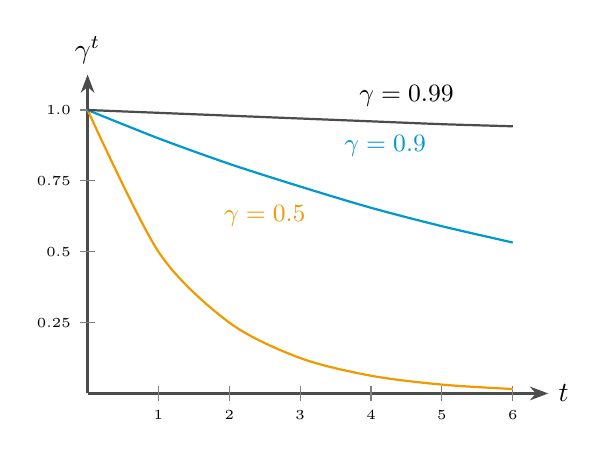
\begin{tikzpicture}[scale=0.9]
    % Axes
    \draw[-{Stealth}, thick, black!70] (0,0) -- (6.5,0) node[right, text=black] {$t$};
    \draw[-{Stealth}, thick, black!70] (0,0) -- (0,4.5) node[above, text=black] {$\gamma^t$};

    % Tick marks
    \foreach \x in {1,2,3,4,5,6} {
        \draw[black!50] (\x,0.1) -- (\x,-0.1) node[below, text=black, font=\tiny] {\x};
    }
    \foreach \y/\ylabel in {1/0.25, 2/0.5, 3/0.75, 4/1.0} {
        \draw[black!50] (0.1,\y) -- (-0.1,\y) node[left, text=black, font=\tiny] {\ylabel};
    }

    % gamma = 0.5 (decays fast)
    \draw[thick, gold] plot[smooth] coordinates {
        (0,4) (1,2) (2,1) (3,0.5) (4,0.25) (5,0.125) (6,0.0625)
    };
    \node[text=gold, font=\small] at (2.5,2.5) {$\gamma = 0.5$};

    % gamma = 0.9 (decays slower)
    \draw[thick, echoblue] plot[smooth] coordinates {
        (0,4) (1,3.6) (2,3.24) (3,2.92) (4,2.62) (5,2.36) (6,2.13)
    };
    \node[text=echoblue, font=\small] at (4.2,3.5) {$\gamma = 0.9$};

    % gamma = 0.99 (almost flat)
    \draw[thick, black!70] plot[smooth] coordinates {
        (0,4) (1,3.96) (2,3.92) (3,3.88) (4,3.84) (5,3.80) (6,3.77)
    };
    \node[text=black, font=\small] at (4.5,4.2) {$\gamma = 0.99$};
\end{tikzpicture}
\caption{The discount factor $\gamma$ controls how quickly rewards are discounted over time. With $\gamma = 0.5$, rewards decay rapidly and the agent is myopic. With $\gamma = 0.99$, rewards decay slowly and the agent plans far into the future.}
\label{fig:discount-decay}
\end{figure}

\marginnote{This rule of thumb comes from the expected value of a geometric distribution with parameter $\gamma$, which governs how far into the future the agent effectively ``looks.''}

There are several reasons to use a discount factor less than 1. First, discounting provides \textbf{mathematical convenience} by ensuring the infinite sum $\sum_{t=0}^{\infty} \gamma^t r_t$ converges to a finite value, which is necessary for the mathematics of infinite-horizon problems to work out cleanly.

Second, discounting models \textbf{uncertainty about the future}. The further we look ahead, the less confident we should be in our predictions. The environment might change, the episode might terminate unexpectedly, or our model of the world might become increasingly inaccurate.

Third, discounting captures a \textbf{preference for sooner rewards}, analogous to the economic concept of time preference. A dollar today is worth more than a dollar tomorrow, both because of opportunity cost (the dollar today can be invested) and because the future is uncertain.

Interestingly, psychological research has found that humans exhibit \textbf{hyperbolic discounting} rather than the exponential discounting ($\gamma^t$) used in standard RL \citep{ainslie1975specious, laibson1997golden}. Humans often prefer \$100 today over \$110 tomorrow, but prefer \$110 in 31 days over \$100 in 30 days. This leads to time inconsistency---optimal decisions appear to change just because time has passed. RL uses exponential discounting precisely because it guarantees \textbf{time consistency}: the optimal policy is the same whether we're planning today or tomorrow.

\begin{figure}[h]
\centering
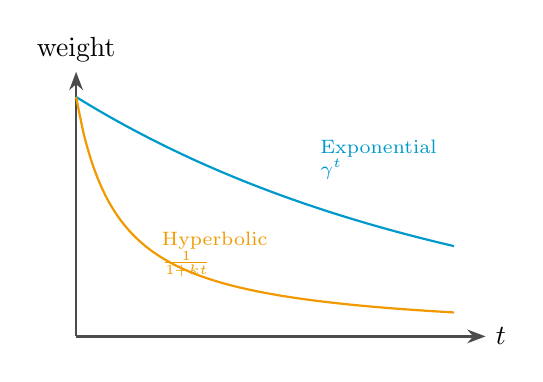
\begin{tikzpicture}[scale=0.8]
    % Axes
    \draw[-{Stealth}, thick, black!70] (0,0) -- (6.5,0) node[right, text=black] {$t$};
    \draw[-{Stealth}, thick, black!70] (0,0) -- (0,4.2) node[above, text=black] {weight};

    % Exponential discounting (gamma = 0.85)
    \draw[thick, echoblue] plot[smooth, domain=0:6, samples=50] (\x, {3.8*0.85^\x});
    \node[text=echoblue, font=\scriptsize, align=left] at (4.8,2.8) {Exponential\\$\gamma^t$};

    % Hyperbolic discounting
    \draw[thick, gold] plot[smooth, domain=0:6, samples=50] (\x, {3.8/(1+1.5*\x)});
    \node[text=gold, font=\scriptsize, align=left] at (2.2,1.3) {Hyperbolic\\$\frac{1}{1+kt}$};
\end{tikzpicture}
\caption{Exponential vs.\ hyperbolic discounting. Hyperbolic discounting (observed in humans) discounts the near-term more steeply but flattens out for distant rewards, leading to time-inconsistent preferences. Exponential discounting maintains a constant rate and guarantees time consistency.}
\label{fig:hyperbolic-discount}
\end{figure}

\subsection{Value Functions}

A \textbf{policy} $\pi: \Sset \to \Aset$ specifies how the agent behaves. For stochastic policies, we write $\pi(a \mid s)$ for the probability of taking action $a$ in state $s$. Our goal is to find an \textbf{optimal policy} $\pi^*$ that maximizes expected cumulative reward.

\begin{definition}[State-Value Function]
The \textbf{state-value function} $V^\pi(s)$ for a policy $\pi$ is the expected return starting from state $s$ and following $\pi$:
\[
V^\pi(s) = \E_\pi \left[ G_t \mid s_t = s \right] = \E_\pi \left[ \sum_{k=0}^{\infty} \gamma^k r_{t+k+1} \mid s_t = s \right]
\]
This function answers: ``How good is it to be in state $s$ when following policy $\pi$?''
\end{definition}

\begin{definition}[Action-Value Function]
The \textbf{action-value function} $Q^\pi(s, a)$ is the expected return starting from state $s$, taking action $a$, and then following $\pi$:
\[
Q^\pi(s, a) = \E_\pi \left[ G_t \mid s_t = s, a_t = a \right]
\]
This function answers: ``How good is it to take action $a$ in state $s$?''
\end{definition}

These two value functions are related by:
\[
V^\pi(s) = \sum_{a} \pi(a \mid s) Q^\pi(s, a)
\]
For a deterministic policy, this simplifies to $V^\pi(s) = Q^\pi(s, \pi(s))$.

\subsection{Optimal Value Functions}

The \textbf{optimal value functions} represent the best possible performance achievable by any policy:
\[
V^*(s) = \max_\pi V^\pi(s), \qquad Q^*(s, a) = \max_\pi Q^\pi(s, a)
\]

A crucial result is that given $Q^*$, the optimal policy has a simple form:
\[
\pi^*(s) = \argmax_{a \in \Aset} Q^*(s, a)
\]
This is why finding $Q^*$ or $V^*$ is the core goal of many RL algorithms---once we have the optimal value function, the optimal policy follows immediately.

\subsection{The Bellman Equations}

Value functions satisfy a fundamental recursive relationship called the \textbf{Bellman equation}, named after Richard Bellman \citep{bellman1957dynamic}. The core idea is:
\begin{center}
\emph{Value now = Immediate reward + Discounted future value}
\end{center}

\begin{theorem}[Bellman Expectation Equation]
For any policy $\pi$, the value function satisfies:
\[
V^\pi(s) = \sum_{a} \pi(a \mid s) \left[ R(s, a) + \gamma \sum_{s'} \T(s' \mid s, a) V^\pi(s') \right]
\]
\end{theorem}

This equation expresses $V^\pi(s)$ as the expected immediate reward plus the discounted expected value of the next state, where the expectations are taken over the policy's action distribution and the environment's transition probabilities.

\begin{theorem}[Bellman Optimality Equation]
The optimal value function satisfies:
\[
V^*(s) = \max_{a \in \Aset} \left[ R(s, a) + \gamma \sum_{s' \in \Sset} \T(s' \mid s, a) V^*(s') \right]
\]
\end{theorem}

\marginnote{The Bellman optimality equation is a system of $|\Sset|$ nonlinear equations due to the $\max$ operator. We cannot solve it directly via matrix inversion, which motivates iterative methods like value iteration.}

The Bellman optimality equation characterizes $V^*$ as a \textbf{fixed point}: if we apply the right-hand side to $V^*$, we get $V^*$ back. Finding this fixed point gives us the optimal value function, from which we can extract the optimal policy.

%%%%%%%%%%%%%%%%%%%%%%%%%%%%%%%%%%%%%%%%%%%%%%%%%%%%%%%%%%%%%%%%%%%%%%%%%%%%%%%
\subsection{Categorizing RL Agents}
%%%%%%%%%%%%%%%%%%%%%%%%%%%%%%%%%%%%%%%%%%%%%%%%%%%%%%%%%%%%%%%%%%%%%%%%%%%%%%%

RL agents can be categorized along several dimensions. \textbf{Value-based} methods learn a value function and derive the policy from it; examples include Q-learning and DQN \citep{mnih2015human}. \textbf{Policy-based} methods learn the policy directly without explicitly representing the value function; examples include REINFORCE \citep{williams1992simple} and PPO \citep{schulman2017proximal}. \textbf{Actor-critic} methods learn both a value function (the critic) and a policy (the actor), using the value function to reduce variance in policy updates.

Another important distinction is between \textbf{model-free} and \textbf{model-based} approaches. Model-free methods learn directly from experience without building an explicit model of the environment's dynamics. Model-based methods learn a model of the transition function and reward function, then use planning algorithms to derive a policy.

Finally, the nature of the state and action spaces matters greatly for algorithm design. \textbf{Tabular} methods represent value functions as tables with one entry per state (or state-action pair), giving exact solutions but requiring small, discrete state spaces. \textbf{Function approximation} methods use parameterized functions (often neural networks) to represent values or policies, enabling generalization across states but introducing approximation error and potential instability.

%%%%%%%%%%%%%%%%%%%%%%%%%%%%%%%%%%%%%%%%%%%%%%%%%%%%%%%%%%%%%%%%%%%%%%%%%%%%%%%
\subsection{Example: Grid World MDP}
%%%%%%%%%%%%%%%%%%%%%%%%%%%%%%%%%%%%%%%%%%%%%%%%%%%%%%%%%%%%%%%%%%%%%%%%%%%%%%%

To make these concepts concrete, consider a grid world environment---a classic testbed for RL algorithms.

\begin{example}[Grid World MDP]
Consider a $4 \times 4$ grid world where the \textbf{state space} $\Sset = \{(x, y) : x, y \in \{0, 1, 2, 3\}\}$ consists of 16 grid positions. The \textbf{action space} $\Aset = \{\uparrow, \downarrow, \leftarrow, \rightarrow\}$ contains four movement directions. Position $(3, 3)$ is a \textbf{goal state} with reward $+10$, while positions $(1, 2)$ and $(2, 1)$ are \textbf{hazard states} with reward $-5$. Each transition incurs a small \textbf{step cost} of $-0.04$, encouraging the agent to reach the goal quickly. The \textbf{discount factor} is $\gamma = 0.9$.
\end{example}

\begin{figure}[h]
\centering
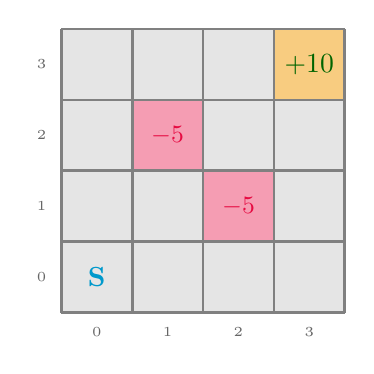
\begin{tikzpicture}[scale=1.0]
    \def\cellsize{0.9}
    % Fill all cells with base color first
    \foreach \x in {0,1,2,3} {
        \foreach \y in {0,1,2,3} {
            \fill[boxgray] (\x*\cellsize, \y*\cellsize) rectangle +(\cellsize, \cellsize);
        }
    }
    % Goal state (top-right) - (3,3)
    \fill[gold!50] (3*\cellsize, 3*\cellsize) rectangle +(\cellsize, \cellsize);
    % Hazard states - (1,2) and (2,1)
    \fill[vividred!40] (1*\cellsize, 2*\cellsize) rectangle +(\cellsize, \cellsize);
    \fill[vividred!40] (2*\cellsize, 1*\cellsize) rectangle +(\cellsize, \cellsize);
    % Draw grid lines on top
    \draw[black!50, line width=1pt, step=\cellsize] (0,0) grid (4*\cellsize, 4*\cellsize);
    % Labels inside cells
    \node[text=olivegreen, font=\bfseries] at (3*\cellsize+\cellsize/2, 3*\cellsize+\cellsize/2) {$+10$};
    \node[text=vividred, font=\small\bfseries] at (1*\cellsize+\cellsize/2, 2*\cellsize+\cellsize/2) {$-5$};
    \node[text=vividred, font=\small\bfseries] at (2*\cellsize+\cellsize/2, 1*\cellsize+\cellsize/2) {$-5$};
    \node[text=echoblue, font=\bfseries] at (\cellsize/2, \cellsize/2) {S};
    % Axis labels
    \foreach \i in {0,1,2,3} {
        \node[text=black!60, font=\tiny] at (-0.25, \i*\cellsize+\cellsize/2) {\i};
        \node[text=black!60, font=\tiny] at (\i*\cellsize+\cellsize/2, -0.25) {\i};
    }
\end{tikzpicture}
\hspace{2cm}
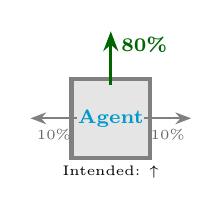
\begin{tikzpicture}[scale=0.85]
    % Center cell
    \node[draw=black!50, fill=boxgray, minimum size=1cm, line width=1.5pt] (center) at (0,0) {};
    \node[text=echoblue, font=\scriptsize\bfseries] at (0,0) {Agent};
    % Intended direction (up) - 80%
    \draw[-{Stealth[length=2.5mm]}, very thick, olivegreen] (0, 0.5) -- (0, 1.3);
    \node[text=olivegreen, font=\scriptsize\bfseries] at (0.5, 1.1) {80\%};
    % Perpendicular (left) - 10%
    \draw[-{Stealth[length=2mm]}, thick, black!50] (-0.5, 0) -- (-1.2, 0);
    \node[text=black!60, font=\tiny] at (-0.85, -0.25) {10\%};
    % Perpendicular (right) - 10%
    \draw[-{Stealth[length=2mm]}, thick, black!50] (0.5, 0) -- (1.2, 0);
    \node[text=black!60, font=\tiny] at (0.85, -0.25) {10\%};
    % Label
    \node[text=black, font=\tiny] at (0, -0.8) {Intended: $\uparrow$};
\end{tikzpicture}
\caption{\emph{Left:} The $4 \times 4$ grid world MDP. The agent starts at S, aims for the goal (+10), and must avoid hazards ($-5$). \emph{Right:} Stochastic ``slippery'' dynamics---the agent moves in the intended direction with 80\% probability, but slips perpendicular with 10\% probability each.}
\label{fig:gridworld}
\end{figure}

The dynamics are \textbf{stochastic} to model real-world uncertainty. With 80\% probability, the agent moves in the intended direction. With 10\% probability each, the agent slips to one of the perpendicular directions. Hitting a wall means staying in place.

For example, if the agent takes action $\uparrow$ in state $s$:
\begin{align*}
\T(s_{\text{above}} \mid s, \uparrow) &= 0.8 \\
\T(s_{\text{left}} \mid s, \uparrow) &= 0.1 \\
\T(s_{\text{right}} \mid s, \uparrow) &= 0.1
\end{align*}

This stochastic dynamics makes the problem interesting: the agent cannot simply plan a shortest path, but must account for the risk of accidentally slipping into hazard states.

How many deterministic policies exist for this small MDP? Each of the 16 states needs an action assignment, with 4 choices per state, giving $|\Aset|^{|\Sset|} = 4^{16} = 4{,}294{,}967{,}296$ deterministic policies---over 4 billion! Even for this tiny MDP, brute-force enumeration is impossible. We need efficient algorithms.


%%%%%%%%%%%%%%%%%%%%%%%%%%%%%%%%%%%%%%%%%%%%%%%%%%%%%%%%%%%%%%%%%%%%%%%%%%%%%%%
\section{Value Iteration}
\label{sec:value-iteration}
%%%%%%%%%%%%%%%%%%%%%%%%%%%%%%%%%%%%%%%%%%%%%%%%%%%%%%%%%%%%%%%%%%%%%%%%%%%%%%%

Given an MDP $(\Sset, \Aset, \T, R, \gamma)$ with known dynamics, how do we compute the optimal policy $\pi^*$? \textbf{Value iteration} is a dynamic programming algorithm that computes the optimal value function by iteratively applying the Bellman optimality operator \citep{bellman1957dynamic}.

Think of $V_k(s)$ as the optimal value if the agent has exactly $k$ steps remaining to act. With no steps remaining, there is no opportunity to collect future reward, so $V_0(s) = 0$ for non-terminal states (terminal states retain their fixed values). For general $k$, the optimal $k$-step value uses optimal $(k{-}1)$-step values:
\[
V_k(s) = \max_a \left[ R(s, a) + \gamma \sum_{s'} \T(s' \mid s, a) V_{k-1}(s') \right]
\]
As $k \to \infty$, this converges to the true optimal value function $V^*$.

\subsection{The Bellman Optimality Operator} 

\begin{definition}[Bellman Optimality Operator]
The \textbf{Bellman optimality operator} $\mathcal{B}: \R^{|\Sset|} \to \R^{|\Sset|}$ is defined as:
\[
(\mathcal{B}V)(s) = \max_{a \in \Aset} \left[ R(s, a) + \gamma \sum_{s' \in \Sset} \T(s' \mid s, a) V(s') \right]
\]
\end{definition}

Value iteration simply applies this operator repeatedly: $V_{k+1} = \mathcal{B}V_k$. Similarly, for a fixed policy $\pi$, we can define the \textbf{Bellman policy operator} $\mathcal{B}^\pi$:
\[
(\mathcal{B}^\pi V)(s) = \sum_{a} \pi(a \mid s) \left[ R(s, a) + \gamma \sum_{s'} \T(s' \mid s, a) V(s') \right]
\]

\subsection{The Algorithm} 

\begin{algorithm}[Value Iteration]
\label{alg:value-iteration}
\begin{enumerate}
    \item \textbf{Initialize:} $V_0(s) = 0$ for all $s \in \Sset$
    \item \textbf{Iterate:} For $k = 0, 1, 2, \ldots$ until convergence:
    \[
    V_{k+1}(s) = \max_{a \in \Aset} \left[ R(s, a) + \gamma \sum_{s' \in \Sset} \T(s' \mid s, a) V_k(s') \right] \quad \forall s \in \Sset
    \]
    \item \textbf{Stopping criterion:} $\|V_{k+1} - V_k\|_\infty < \epsilon$ for some threshold $\epsilon > 0$
    \item \textbf{Extract policy:}
    \[
    \pi^*(s) = \argmax_{a \in \Aset} \left[ R(s, a) + \gamma \sum_{s'} \T(s' \mid s, a) V^*(s') \right]
    \]
\end{enumerate}
\end{algorithm}

\subsection{A Worked Example}

Let's trace through value iteration on our grid world. We treat terminal states (goal and hazards) as absorbing states with fixed values: $V(\text{goal}) = 10$ and $V(\text{hazard}) = -5$. All non-terminal states are initialized to $V_0(s) = 0$. 

\begin{figure}[h]
\centering
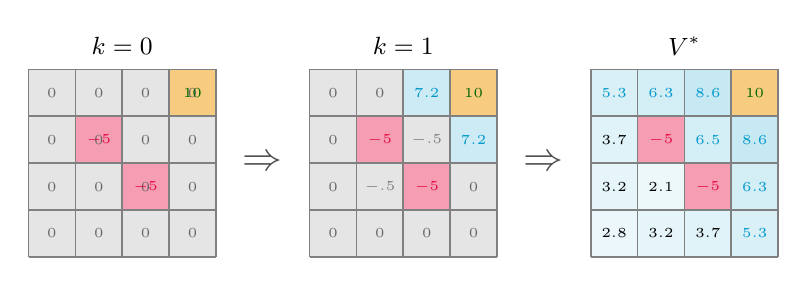
\begin{tikzpicture}[scale=0.85]
    \def\s{0.7}
    
    % ===== Grid 1: k=0 =====
    \node[text=black, font=\small\bfseries] at (2*\s, 4.5*\s) {$k=0$};
    % Base fill
    \foreach \x in {0,1,2,3} { \foreach \y in {0,1,2,3} {
        \fill[boxgray] (\x*\s, \y*\s) rectangle +(\s, \s);
    }}
    % Special cells
    \fill[gold!50] (3*\s, 3*\s) rectangle +(\s, \s);
    \fill[vividred!40] (1*\s, 2*\s) rectangle +(\s, \s);
    \fill[vividred!40] (2*\s, 1*\s) rectangle +(\s, \s);
    % Grid lines
    \draw[black!50, line width=0.6pt, step=\s] (0,0) grid (4*\s, 4*\s);
    % Values
    \foreach \x in {0,1,2,3} { \foreach \y in {0,1,2,3} {
        \node[text=black!60, font=\tiny] at (\x*\s+\s/2, \y*\s+\s/2) {$0$};
    }}
    % Overwrite terminal states
    \node[text=olivegreen, font=\tiny\bfseries] at (3*\s+\s/2, 3*\s+\s/2) {$10$};
    \node[text=vividred, font=\tiny] at (1*\s+\s/2, 2*\s+\s/2) {$-5$};
    \node[text=vividred, font=\tiny] at (2*\s+\s/2, 1*\s+\s/2) {$-5$};
    
    % Arrow
    \node[text=black!70, font=\Large] at (5*\s, 2*\s) {$\Rightarrow$};
    
    % ===== Grid 2: k=1 =====
    \def\ox{6}
    \node[text=black, font=\small\bfseries] at (\ox*\s+2*\s, 4.5*\s) {$k=1$};
    % Base fill
    \foreach \x in {0,1,2,3} { \foreach \y in {0,1,2,3} {
        \fill[boxgray] (\ox*\s+\x*\s, \y*\s) rectangle +(\s, \s);
    }}
    % Highlight updated cells
    \fill[echoblue!20] (\ox*\s+2*\s, 3*\s) rectangle +(\s, \s);
    \fill[echoblue!20] (\ox*\s+3*\s, 2*\s) rectangle +(\s, \s);
    % Special cells
    \fill[gold!50] (\ox*\s+3*\s, 3*\s) rectangle +(\s, \s);
    \fill[vividred!40] (\ox*\s+1*\s, 2*\s) rectangle +(\s, \s);
    \fill[vividred!40] (\ox*\s+2*\s, 1*\s) rectangle +(\s, \s);
    % Grid lines
    \foreach \i in {0,1,2,3,4} {
        \draw[black!50, line width=0.6pt] (\ox*\s+\i*\s, 0) -- (\ox*\s+\i*\s, 4*\s);
        \draw[black!50, line width=0.6pt] (\ox*\s, \i*\s) -- (\ox*\s+4*\s, \i*\s);
    }
    % Values
    \foreach \x/\y in {0/0,1/0,2/0,3/0,0/1,3/1,0/2,0/3,1/3} {
        \node[text=black!60, font=\tiny] at (\ox*\s+\x*\s+\s/2, \y*\s+\s/2) {$0$};
    }
    \node[text=black!50, font=\tiny] at (\ox*\s+1*\s+\s/2, 1*\s+\s/2) {$-.5$};
    \node[text=black!50, font=\tiny] at (\ox*\s+2*\s+\s/2, 2*\s+\s/2) {$-.5$};
    \node[text=echoblue, font=\tiny\bfseries] at (\ox*\s+2*\s+\s/2, 3*\s+\s/2) {$7.2$};
    \node[text=echoblue, font=\tiny\bfseries] at (\ox*\s+3*\s+\s/2, 2*\s+\s/2) {$7.2$};
    \node[text=olivegreen, font=\tiny\bfseries] at (\ox*\s+3*\s+\s/2, 3*\s+\s/2) {$10$};
    \node[text=vividred, font=\tiny] at (\ox*\s+1*\s+\s/2, 2*\s+\s/2) {$-5$};
    \node[text=vividred, font=\tiny] at (\ox*\s+2*\s+\s/2, 1*\s+\s/2) {$-5$};
    
    % Arrow
    \node[text=black!70, font=\Large] at (11*\s, 2*\s) {$\Rightarrow$};
    
    % ===== Grid 3: Converged =====
    \def\oxx{12}
    \node[text=black, font=\small\bfseries] at (\oxx*\s+2*\s, 4.5*\s) {$V^*$};
    % Base fill with value-based coloring
    \foreach \x/\y/\c in {0/0/8,1/0/10,2/0/12,3/0/15,0/1/10,1/1/7,3/1/17,0/2/12,2/2/17,3/2/22,0/3/15,1/3/17,2/3/22} {
        \fill[echoblue!\c] (\oxx*\s+\x*\s, \y*\s) rectangle +(\s, \s);
    }
    % Special cells
    \fill[gold!50] (\oxx*\s+3*\s, 3*\s) rectangle +(\s, \s);
    \fill[vividred!40] (\oxx*\s+1*\s, 2*\s) rectangle +(\s, \s);
    \fill[vividred!40] (\oxx*\s+2*\s, 1*\s) rectangle +(\s, \s);
    % Grid lines
    \foreach \i in {0,1,2,3,4} {
        \draw[black!50, line width=0.6pt] (\oxx*\s+\i*\s, 0) -- (\oxx*\s+\i*\s, 4*\s);
        \draw[black!50, line width=0.6pt] (\oxx*\s, \i*\s) -- (\oxx*\s+4*\s, \i*\s);
    }
    % Converged values
    \node[text=black, font=\tiny] at (\oxx*\s+0*\s+\s/2, 0*\s+\s/2) {$2.8$};
    \node[text=black, font=\tiny] at (\oxx*\s+1*\s+\s/2, 0*\s+\s/2) {$3.2$};
    \node[text=black, font=\tiny] at (\oxx*\s+2*\s+\s/2, 0*\s+\s/2) {$3.7$};
    \node[text=echoblue, font=\tiny] at (\oxx*\s+3*\s+\s/2, 0*\s+\s/2) {$5.3$};
    \node[text=black, font=\tiny] at (\oxx*\s+0*\s+\s/2, 1*\s+\s/2) {$3.2$};
    \node[text=black, font=\tiny] at (\oxx*\s+1*\s+\s/2, 1*\s+\s/2) {$2.1$};
    \node[text=vividred, font=\tiny\bfseries] at (\oxx*\s+2*\s+\s/2, 1*\s+\s/2) {$-5$};
    \node[text=echoblue, font=\tiny] at (\oxx*\s+3*\s+\s/2, 1*\s+\s/2) {$6.3$};
    \node[text=black, font=\tiny] at (\oxx*\s+0*\s+\s/2, 2*\s+\s/2) {$3.7$};
    \node[text=vividred, font=\tiny\bfseries] at (\oxx*\s+1*\s+\s/2, 2*\s+\s/2) {$-5$};
    \node[text=echoblue, font=\tiny] at (\oxx*\s+2*\s+\s/2, 2*\s+\s/2) {$6.5$};
    \node[text=echoblue, font=\tiny\bfseries] at (\oxx*\s+3*\s+\s/2, 2*\s+\s/2) {$8.6$};
    \node[text=echoblue, font=\tiny] at (\oxx*\s+0*\s+\s/2, 3*\s+\s/2) {$5.3$};
    \node[text=echoblue, font=\tiny] at (\oxx*\s+1*\s+\s/2, 3*\s+\s/2) {$6.3$};
    \node[text=echoblue, font=\tiny\bfseries] at (\oxx*\s+2*\s+\s/2, 3*\s+\s/2) {$8.6$};
    \node[text=olivegreen, font=\tiny\bfseries] at (\oxx*\s+3*\s+\s/2, 3*\s+\s/2) {$10$};
\end{tikzpicture}
\caption{Value iteration progression on the grid world. \emph{Left ($k=0$):} Initial values are zero for non-terminal states; terminal states have fixed values. \emph{Center ($k=1$):} After one iteration, states adjacent to the goal receive positive values (highlighted); states near hazards receive negative values. \emph{Right ($V^*$):} Converged values after $\sim$16 iterations, with color intensity indicating value magnitude. Values ``flow'' outward from the goal.}
\label{fig:value-iteration-progression}
\end{figure}

\marginnote[-2cm]{In this simplified formulation, terminal state values are fixed and the step cost is absorbed into the terminal rewards. This is pedagogically convenient but differs slightly from the general Bellman formulation where $R(s,a)$ appears explicitly.}

\noindent Consider state $(2, 3)$, which is adjacent to the goal. The best action is $\rightarrow$ (moving right toward the goal). Applying the Bellman backup:
\begin{align*}
V_1(2,3) &= \max_a \gamma \sum_{s'} \T(s' \mid (2,3), a) \cdot V_0(s') \\
&= 0.9 \times \left[ \underbrace{0.8 \cdot 10}_{\text{reach goal}} + \underbrace{0.1 \cdot 0}_{\text{slip up}} + \underbrace{0.1 \cdot 0}_{\text{slip down}} \right] \\
&= 0.9 \times 8 = 7.2
\end{align*}

State $(1, 1)$ is adjacent to both hazards. Its best action (moving away from hazards) still risks slipping into one:
\[
V_1(1,1) = 0.9 \times (0.8 \cdot 0 + 0.1 \cdot 0 + 0.1 \cdot (-5)) = 0.9 \times (-0.5) = -0.45 \approx -0.5
\]

After convergence (approximately 16 iterations for $\gamma = 0.9$), the value function shows how ``value flows'' from the goal outward. States closer to the goal with safer paths have higher values. State $(1,1)$ has lower value than its neighbors because it is adjacent to both hazards. The optimal policy follows the value gradient toward the goal while avoiding hazards.

\begin{figure}[h]
\centering
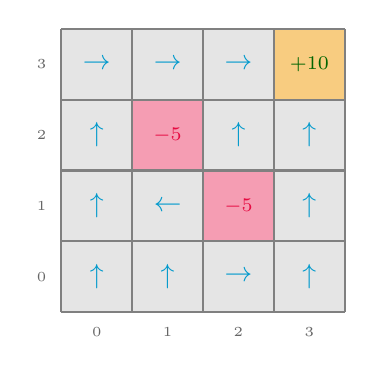
\begin{tikzpicture}[scale=1.0]
    \def\s{0.9}
    % Fill all cells with background
    \foreach \x in {0,1,2,3} { \foreach \y in {0,1,2,3} {
        \fill[boxgray] (\x*\s, \y*\s) rectangle +(\s, \s);
    }}
    % Goal state
    \fill[gold!50] (3*\s, 3*\s) rectangle +(\s, \s);
    % Hazard states
    \fill[vividred!40] (1*\s, 2*\s) rectangle +(\s, \s);
    \fill[vividred!40] (2*\s, 1*\s) rectangle +(\s, \s);
    % Grid lines
    \draw[black!50, line width=0.8pt, step=\s] (0,0) grid (4*\s, 4*\s);
    % Goal/Hazard labels
    \node[text=olivegreen, font=\scriptsize\bfseries] at (3*\s+\s/2, 3*\s+\s/2) {$+10$};
    \node[text=vividred, font=\scriptsize\bfseries] at (1*\s+\s/2, 2*\s+\s/2) {$-5$};
    \node[text=vividred, font=\scriptsize\bfseries] at (2*\s+\s/2, 1*\s+\s/2) {$-5$};
    % Optimal policy arrows
    % Row 3 (top)
    \node[text=echoblue, font=\normalsize] at (0*\s+\s/2, 3*\s+\s/2) {$\rightarrow$};
    \node[text=echoblue, font=\normalsize] at (1*\s+\s/2, 3*\s+\s/2) {$\rightarrow$};
    \node[text=echoblue, font=\normalsize] at (2*\s+\s/2, 3*\s+\s/2) {$\rightarrow$};
    % Row 2
    \node[text=echoblue, font=\normalsize] at (0*\s+\s/2, 2*\s+\s/2) {$\uparrow$};
    \node[text=echoblue, font=\normalsize] at (2*\s+\s/2, 2*\s+\s/2) {$\uparrow$};
    \node[text=echoblue, font=\normalsize] at (3*\s+\s/2, 2*\s+\s/2) {$\uparrow$};
    % Row 1
    \node[text=echoblue, font=\normalsize] at (0*\s+\s/2, 1*\s+\s/2) {$\uparrow$};
    \node[text=echoblue, font=\normalsize] at (1*\s+\s/2, 1*\s+\s/2) {$\leftarrow$};
    \node[text=echoblue, font=\normalsize] at (3*\s+\s/2, 1*\s+\s/2) {$\uparrow$};
    % Row 0 (bottom)
    \node[text=echoblue, font=\normalsize] at (0*\s+\s/2, 0*\s+\s/2) {$\uparrow$};
    \node[text=echoblue, font=\normalsize] at (1*\s+\s/2, 0*\s+\s/2) {$\uparrow$};
    \node[text=echoblue, font=\normalsize] at (2*\s+\s/2, 0*\s+\s/2) {$\rightarrow$};
    \node[text=echoblue, font=\normalsize] at (3*\s+\s/2, 0*\s+\s/2) {$\uparrow$};
    % Axis labels
    \foreach \i in {0,1,2,3} {
        \node[text=black!60, font=\tiny] at (\i*\s+\s/2, -0.25) {\i};
        \node[text=black!60, font=\tiny] at (-0.25, \i*\s+\s/2) {\i};
    }
\end{tikzpicture}
\caption{The optimal policy for the grid world MDP after value iteration converges. Arrows indicate the best action in each state. The policy routes the agent toward the goal while avoiding states adjacent to hazards where possible. Note how state $(1,1)$ moves left to avoid the hazard at $(2,1)$, even though moving up would be shorter.}
\label{fig:gridworld-policy}
\end{figure}

\subsection{Convergence Analysis}

Why does value iteration converge? The answer lies in the \textbf{contraction mapping theorem}.

\begin{theorem}[Bellman Operator is a Contraction]
\label{thm:contraction}
For discount factor $\gamma \in [0, 1)$ and all $V, V' \in \R^{|\Sset|}$:
\[
\|\mathcal{B}V - \mathcal{B}V'\|_\infty \leq \gamma \|V - V'\|_\infty
\]
\end{theorem}

\begin{proof}
For all $s \in \Sset$:
\begin{align*}
(\mathcal{B}V)(s) - (\mathcal{B}V')(s) &= \max_{a} \left[ R(s,a) + \gamma \sum_{s'} \T(s' \mid s,a) V(s') \right] \\
&\quad - \max_{a} \left[ R(s,a) + \gamma \sum_{s'} \T(s' \mid s,a) V'(s') \right]
\end{align*}
Using the fact that $\max_a f(a) - \max_a g(a) \leq \max_a [f(a) - g(a)]$:
\begin{align*}
&\leq \max_{a} \left[ \gamma \sum_{s'} \T(s' \mid s,a) \left( V(s') - V'(s') \right) \right] \\
&\leq \gamma \max_{a} \sum_{s'} \T(s' \mid s,a) \|V - V'\|_\infty \\
&= \gamma \|V - V'\|_\infty
\end{align*}
The last step uses $\sum_{s'} \T(s' \mid s,a) = 1$. Taking the max over $s$ gives the result.
\end{proof}

\begin{theorem}[Convergence of Value Iteration]
For $\gamma \in [0, 1)$, the sequence $V_0, V_1, \ldots$ with $V_{k+1} = \mathcal{B}V_k$ converges to $V^*$.
\end{theorem}

\begin{proof}
The optimal value function $V^*$ is the unique fixed point of $\mathcal{B}$, satisfying $V^* = \mathcal{B}V^*$. For each $k$:
\[
\|V^* - V_{k+1}\|_\infty = \|\mathcal{B}V^* - \mathcal{B}V_k\|_\infty \leq \gamma \|V^* - V_k\|_\infty
\]
By induction:
\[
\|V^* - V_k\|_\infty \leq \gamma^k \|V^* - V_0\|_\infty \to 0 \text{ as } k \to \infty
\]
\end{proof}

\begin{frontiers}
When developing new RL algorithms, contraction mappings provide a powerful tool for building intuition and proving convergence. If you can show your update operator ``shrinks'' the distance between any two value functions (or policies), convergence to a unique fixed point is guaranteed.

This principle extends beyond value iteration. \textbf{Trust Region Policy Optimization (TRPO)} \citep{schulman2015trpo} and \textbf{Proximal Policy Optimization (PPO)} \citep{schulman2017proximal} rely on constraints that limit how much the policy can change in each update---ensuring that performance improves monotonically. While not strictly contraction mappings in the classical sense, these methods embody the same intuition: by controlling the ``step size'' of updates, we can guarantee that each iteration brings us closer to (or at least no further from) the optimal solution.

When designing your own algorithms, ask: \emph{Can I bound how much my update changes the current solution? Does my update operator have a unique fixed point?} Affirmative answers often lead to provable convergence guarantees.
\end{frontiers}

\marginnote{The convergence rate is \textbf{geometric}: the error decreases by a factor of $\gamma$ each iteration. For $\gamma = 0.9$, approximately 44 iterations reduce the error by a factor of 100.}

Value iteration converges under two conditions: either $\gamma < 1$, or all policies eventually reach a terminal state.

\subsection{Asynchronous Value Iteration}

A remarkable property of value iteration is that it converges even when states are updated \textbf{asynchronously}---different states can be updated at different times, even using outdated values.

\begin{theorem}[Asynchronous Convergence]
Fix a finite MDP $(\Sset, \Aset, \T, R)$ and $\gamma \in [0, 1)$. If $\Sset_0, \Sset_1, \ldots$ is a sequence of state subsets such that each state $s \in \Sset$ appears infinitely often, then the sequence generated by
\[
V_{k+1}(s) = \begin{cases}
(\mathcal{B}V_k)(s) & s \in \Sset_k \\
V_k(s) & s \notin \Sset_k
\end{cases}
\]
converges to $V^*$ for any initialization $V_0$.
\end{theorem}

\begin{proof}[Proof sketch]
Since $\mathcal{B}$ is a $\gamma$-contraction, for any updated state $s \in \Sset_k$:
\[
|V^*(s) - V_{k+1}(s)| = |(\mathcal{B}V^*)(s) - (\mathcal{B}V_k)(s)| \leq \gamma \|V^* - V_k\|_\infty
\]
Because each state appears infinitely often, the error eventually contracts for all states, and the sequence converges to $V^*$.
\end{proof}

This theorem has important practical implications. \textbf{Gauss-Seidel value iteration} updates states in sequence, using newly computed values immediately. When computing $V(s_i)$, it uses already-updated values $V(s_1), \ldots, V(s_{i-1})$. This often converges faster because information propagates within a single sweep.

\textbf{Parallel value iteration} allows different processors to update different states simultaneously, enabling efficient distributed implementations. This is especially important for modern RL with large language models, where computational throughput is paramount.

\textbf{Prioritized sweeping} focuses updates on states with large Bellman errors, potentially achieving faster convergence by updating the most ``out-of-date'' states first.

\begin{frontiers}
It's worth nothing the importance of asynchronous updates. Just like in value iteration, asynchronous updates have shown great success in modern deep RL. More recently, \textbf{PipelineRL} \citep{piche2025pipelinerl} takes asynchronicity further by overlapping different stages of the learning pipeline---data collection, gradient computation, and parameter updates can proceed simultaneously on different hardware.
This has been validated as a key way to improve convergence speed (at least in wall clock time)in large scale recipe experiments by \citet{khatri2025scalerl}.
But these weren't the first to try and make async RL work well in deep RL, methods like \textbf{IMPALA} \citep{espeholt2018impala}, \textbf{Ape-X} \citep{horgan2018distributed}, and \textbf{Asynchronous Advantage Actor-Critic (A3C/A2C)} \citep{mnih2016asynchronous} use this approach to achieve orders-of-magnitude (wall clock) speedups over synchronous training at the cost of some stability issues and engineering challenges.
\end{frontiers}

\subsection{Implementation}

Here is a Python implementation of value iteration:

\begin{lstlisting}[language=Python, caption={Value Iteration Implementation}]
import numpy as np

class ValueIteration:
    """Standard Value Iteration algorithm for MDPs."""

    def __init__(self, mdp):
        self.mdp = mdp

    def run(self, theta=0.001, gamma=0.9):
        """Run value iteration until convergence."""
        V = np.zeros(self.mdp.S)
        
        while True:
            delta = 0
            V_old = V.copy()

            for s in range(self.mdp.S):
                q_values = []
                for a in range(self.mdp.A):
                    q = self.mdp.R[s, a] + gamma * sum(
                        self.mdp.T[s, a, sp] * V_old[sp] 
                        for sp in range(self.mdp.S))
                    q_values.append(q)
                
                V[s] = max(q_values)
                delta = max(delta, abs(V_old[s] - V[s]))

            if delta < theta:
                break

        pi = self.get_policy(V, gamma)
        return pi, V

    def get_policy(self, V, gamma=0.9):
        """Extract greedy policy from value function."""
        pi = {}
        for s in range(self.mdp.S):
            q_values = [
                self.mdp.R[s, a] + gamma * sum(
                    self.mdp.T[s, a, sp] * V[sp] 
                    for sp in range(self.mdp.S))
                for a in range(self.mdp.A)]
            pi[s] = np.argmax(q_values)
        return pi
\end{lstlisting}

The standard implementation above uses \textbf{synchronous} (or \textbf{Jacobi-style}) updates: all states are updated using the values from the previous iteration. An alternative is \textbf{Gauss-Seidel} updates, where we use newly computed values immediately within the same sweep.

\begin{lstlisting}[language=Python, caption={Gauss-Seidel Value Iteration}]
class GaussSeidelValueIteration:
    """Gauss-Seidel VI: use updated values immediately."""

    def __init__(self, mdp):
        self.mdp = mdp

    def run(self, theta=0.001, gamma=0.9):
        V = np.zeros(self.mdp.S)
        
        while True:
            delta = 0
            # Key difference: NO copy - use V directly
            for s in range(self.mdp.S):
                v_old = V[s]
                q_values = []
                for a in range(self.mdp.A):
                    # Uses already-updated V[s'] for s' < s
                    q = self.mdp.R[s, a] + gamma * sum(
                        self.mdp.T[s, a, sp] * V[sp] 
                        for sp in range(self.mdp.S))
                    q_values.append(q)
                V[s] = max(q_values)
                delta = max(delta, abs(v_old - V[s]))

            if delta < theta:
                break
        return V
\end{lstlisting}

Gauss-Seidel updates often converge faster because information propagates within a single sweep rather than waiting for the next iteration. However, the update order can affect convergence speed.

A more sophisticated variant handles \textbf{self-loops} explicitly. When a state can transition back to itself, the standard update mixes old and new values. The \textbf{Jacobi update with self-loop correction} solves for the fixed point analytically:

\begin{lstlisting}[language=Python, caption={Jacobi Value Iteration with Self-Loop Handling}]
class JacobiValueIteration:
    """Jacobi VI with explicit self-loop handling."""

    def __init__(self, mdp):
        self.mdp = mdp

    def run(self, theta=0.001, gamma=0.9):
        V = np.zeros(self.mdp.S)
        
        while True:
            delta = 0
            V_old = V.copy()

            for s in range(self.mdp.S):
                v = V_old[s]
                q_values = []
                for a in range(self.mdp.A):
                    # Separate self-loop from other transitions
                    sum_others = sum(
                        self.mdp.T[s, a, sp] * V_old[sp] 
                        for sp in range(self.mdp.S) if sp != s)
                    # Solve: V(s) = R + gamma*(T[s,a,s]*V(s) + sum_others)
                    # => V(s)*(1 - gamma*T[s,a,s]) = R + gamma*sum_others
                    denom = 1.0 - gamma * self.mdp.T[s, a, s]
                    if denom > 0:
                        q = (self.mdp.R[s, a] + gamma * sum_others) / denom
                    else:
                        q = self.mdp.R[s, a] + gamma * sum_others
                    q_values.append(q)
                V[s] = max(q_values)
                delta = max(delta, abs(v - V[s]))

            if delta < theta:
                break
        return V
\end{lstlisting}

For large MDPs, \textbf{prioritized sweeping} can dramatically improve convergence by focusing computation on states with large Bellman errors:

\begin{lstlisting}[language=Python, caption={Prioritized Sweeping Value Iteration}]
import heapq

class PrioritizedSweepingVI:
    """VI with prioritized state updates."""

    def __init__(self, mdp):
        self.mdp = mdp
        # Build predecessor graph for efficient updates
        self.predecessors = {s: set() for s in range(mdp.S)}
        for s in range(mdp.S):
            for a in range(mdp.A):
                for sp in range(mdp.S):
                    if mdp.T[s, a, sp] > 0:
                        self.predecessors[sp].add(s)

    def run(self, theta=0.0001, gamma=0.9, max_iter=2000):
        V = np.zeros(self.mdp.S)
        # Priority queue: (-priority, state)
        pq = []
        in_queue = set()
        
        # Initialize with Bellman errors
        for s in range(self.mdp.S):
            error = self._bellman_error(s, V, gamma)
            if error > theta:
                heapq.heappush(pq, (-error, s))
                in_queue.add(s)

        for _ in range(max_iter):
            if not pq:
                break
            _, s = heapq.heappop(pq)
            in_queue.discard(s)
            
            # Update V[s]
            V[s] = self._bellman_update(s, V, gamma)
            
            # Add predecessors with large errors to queue
            for p in self.predecessors[s]:
                error = self._bellman_error(p, V, gamma)
                if error > theta and p not in in_queue:
                    heapq.heappush(pq, (-error, p))
                    in_queue.add(p)
        return V

    def _bellman_update(self, s, V, gamma):
        return max(self.mdp.R[s, a] + gamma * sum(
            self.mdp.T[s, a, sp] * V[sp] for sp in range(self.mdp.S))
            for a in range(self.mdp.A))

    def _bellman_error(self, s, V, gamma):
        return abs(V[s] - self._bellman_update(s, V, gamma))
\end{lstlisting}

Prioritized sweeping is particularly effective when value changes are localized---updating one state primarily affects its neighbors. By maintaining a priority queue ordered by Bellman error magnitude, we focus computation where it matters most.

%%%%%%%%%%%%%%%%%%%%%%%%%%%%%%%%%%%%%%%%%%%%%%%%%%%%%%%%%%%%%%%%%%%%%%%%%%%%%%%
\section{Policy Iteration}
\label{sec:policy-iteration}
%%%%%%%%%%%%%%%%%%%%%%%%%%%%%%%%%%%%%%%%%%%%%%%%%%%%%%%%%%%%%%%%%%%%%%%%%%%%%%%

\textbf{Policy iteration}, introduced by \citet{howard1960dynamic}, is an alternative dynamic programming algorithm that alternates between two steps: \textbf{policy evaluation} (computing $V^\pi$ for the current policy) and \textbf{policy improvement} (finding a better policy using the current value function).

\subsection{Overview}

Policy iteration proceeds as follows. First, initialize with an arbitrary policy $\pi_0$. Then, in the \textbf{policy evaluation} step, compute $V^{\pi_i}$ for the current policy. Next, in the \textbf{policy improvement} step, compute a better policy $\pi_{i+1}$ by acting greedily with respect to $V^{\pi_i}$. Repeat until the policy stops changing.

\subsection{Policy Evaluation}

The policy evaluation step requires computing $V^\pi(s)$ for all states. For a fixed policy $\pi$, the Bellman expectation equation becomes:
\[
V^\pi(s) = R(s, \pi(s)) + \gamma \sum_{s'} \T(s' \mid s, \pi(s)) V^\pi(s')
\]
This is a system of $|\Sset|$ linear equations (no $\max$ operator), which can be solved in two ways.

The \textbf{iterative method} applies the Bellman policy operator repeatedly:
\[
V_{k+1}^\pi = R^\pi + \gamma \T^\pi V_k^\pi
\]
This converges because the policy operator $\mathcal{B}^\pi$ is also a $\gamma$-contraction.

The \textbf{direct method} solves the linear system exactly. In matrix form, $V^\pi = R^\pi + \gamma \T^\pi V^\pi$, which gives:
\[
V^\pi = (I - \gamma \T^\pi)^{-1} R^\pi
\]
This is exact but requires $O(|\Sset|^3)$ time for the matrix inversion.

\subsection{Policy Improvement}

Given $V^{\pi_i}$, we construct a new policy that is greedy with respect to the current value function. First, compute $Q^{\pi_i}(s, a)$ for all states and actions:
\[
Q^{\pi_i}(s, a) = R(s, a) + \gamma \sum_{s'} \T(s' \mid s, a) V^{\pi_i}(s')
\]
Then, define the improved policy:
\[
\pi_{i+1}(s) = \argmax_a Q^{\pi_i}(s, a) \quad \forall s \in \Sset
\]

The intuition is straightforward: if taking action $a$ and then following $\pi_i$ yields higher value than just following $\pi_i$ from the start, we should take action $a$.

\subsection{Convergence}

\begin{theorem}[Policy Improvement Theorem]
Let $\pi$ be a policy and $\pi'$ be the greedy policy with respect to $V^\pi$. Then $V^{\pi'}(s) \geq V^\pi(s)$ for all $s \in \Sset$, with equality if and only if $\pi$ is already optimal.
\end{theorem}

\begin{proof}
For any state $s$:
\begin{align*}
V^\pi(s) &\leq \max_a Q^\pi(s, a) = Q^\pi(s, \pi'(s)) \\
&= R(s, \pi'(s)) + \gamma \sum_{s'} \T(s' \mid s, \pi'(s)) V^\pi(s') \\
&\leq R(s, \pi'(s)) + \gamma \sum_{s'} \T(s' \mid s, \pi'(s)) \max_{a'} Q^\pi(s', a') \\
&= R(s, \pi'(s)) + \gamma \sum_{s'} \T(s' \mid s, \pi'(s)) Q^\pi(s', \pi'(s'))
\end{align*}
Continuing this expansion:
\[
V^\pi(s) \leq \E_{\pi'}\left[ \sum_{t=0}^\infty \gamma^t r_{t+1} \mid s_0 = s \right] = V^{\pi'}(s)
\]
\end{proof}

\begin{theorem}[Convergence of Policy Iteration]
Policy iteration converges to the optimal policy $\pi^*$ in a finite number of iterations.
\end{theorem}

\begin{proof}
By the policy improvement theorem, each iteration produces a policy that is at least as good as the previous one. Since there are only finitely many deterministic policies ($|\Aset|^{|\Sset|}$), and each improvement is strict unless we've reached optimality, the algorithm must terminate at $\pi^*$.
\end{proof}

\marginnote{In practice, policy iteration often converges in far fewer iterations than value iteration---sometimes just 2--3 iterations for small MDPs---because each iteration makes ``larger'' improvements by fully evaluating the current policy.}

\subsection{Implementation}

\begin{lstlisting}[language=Python, caption={Policy Iteration Implementation}]
import numpy as np

def policy_iteration(mdp, gamma=0.9, epsilon=0.01):
    """Standard Policy Iteration algorithm."""
    V = np.zeros(mdp.S)
    policy = [0] * mdp.S
    
    while True:
        # Policy Evaluation
        while True:
            delta = 0.0
            for s in range(mdp.S):
                v = V[s]
                a = policy[s]
                V[s] = mdp.R[s, a] + gamma * sum(
                    mdp.T[s, a, sp] * V[sp] for sp in range(mdp.S))
                delta = max(delta, abs(v - V[s]))
            if delta < epsilon:
                break
                
        # Policy Improvement
        policy_stable = True
        for s in range(mdp.S):
            old_action = policy[s]
            q_values = [
                mdp.R[s, a] + gamma * sum(
                    mdp.T[s, a, sp] * V[sp] for sp in range(mdp.S))
                for a in range(mdp.A)]
            policy[s] = np.argmax(q_values)
            if old_action != policy[s]:
                policy_stable = False
                
        if policy_stable:
            return V, policy
\end{lstlisting}

\subsection{Value Iteration vs.\ Policy Iteration}

Both algorithms find the optimal policy, but they have different trade-offs. Value iteration has cost $O(|\Sset|^2 |\Aset|)$ per iteration and requires many iterations (geometric convergence), but uses only $O(|\Sset|)$ memory and is easy to parallelize with asynchronous updates. Policy iteration has cost $O(|\Sset|^3)$ per iteration for exact evaluation (or $O(|\Sset|^2 |\Aset|)$ for iterative evaluation) but requires few iterations (finite, often 2--10). It uses $O(|\Sset|^2)$ memory for exact evaluation and is harder to parallelize.

\paragraph{Strong Polynomiality.}
A deeper theoretical distinction concerns \textbf{strong polynomiality}---whether an algorithm can find an \emph{exactly} optimal policy with computation polynomial in $|\Sset|$, $|\Aset|$, and $1/(1-\gamma)$, without dependence on a precision parameter $\delta$. \citet{ye2011simplex} proved that policy iteration is strongly polynomial, computing an optimal policy with $O(\text{poly}(|\Sset|, |\Aset|, 1/(1-\gamma)))$ arithmetic operations. \citet{scherrer2016improved} later provided a simpler proof showing that policy iteration terminates after at most $O(|\Sset||\Aset|/(1-\gamma))$ iterations.

\marginnote{The RL Theory lecture notes by Csaba Szepesvári \citep{szepesvari2024rltheory} provide an excellent treatment of these complexity results; we follow their exposition here. Available at \url{https://rltheory.github.io/}.}

In contrast, \citet{feinberg2014modified} showed that value iteration is \emph{not} strongly polynomial: there exist MDPs with just three states and two actions where value iteration requires arbitrarily many iterations to find the optimal policy exactly. The intuition is that value iteration can ``hug'' a suboptimal action indefinitely as values approach their limits asymptotically. Policy iteration avoids this by making discrete jumps between policies, allowing it to ``snap'' into the optimal solution.

\paragraph{Practical Implications.} 
Does this theoretical gap matter in practice? Often not. Value iteration achieves $\delta$-suboptimal policies with cost growing only as $\log(1/\delta)$, which is quite mild. Moreover, in real applications we face sampling noise, function approximation error, and model mismatch---all of which make exact optimality unattainable anyway. As \citet{scherrer2016improved} notes, ``exact optimality is nice to have, but approximate computations with runtime growing mildly with the required precision should be almost equally acceptable.''

In practice, \textbf{modified policy iteration} offers a middle ground: perform only a few iterations of policy evaluation (rather than running to convergence) before each policy improvement step. This combines the fast convergence of policy iteration with the computational efficiency of value iteration.


\bibliographystyle{plainnat} 
\bibliography{references}

\end{document}                          %  